\Chapter{Tervezés}

\Section{Bevezetés}

A dolgozat által vizsgált témahoz egy komplex multifunkciós szoftver került megterve\hyp{}zésre, mely a dolgozati téma elemzési részében kifejezetten nagy szerepet tölt be. Összetettsége révén rengeteg időt és odafigyelést igényelt már maga a tervezési fázis is. Számos ábra és tervezet került megalkotásra, melynek a túlnyomó része rendkívül jelentősnek bizonyult az implementáció során.

A legmagasabb szinten az alábbi ábra nyújta a legtisztább áttekintését a különböző funkcióknak és a szoftver sokszínűségének.

\begin{figure}[h!]
\begin{center}
\caption{\textbf{High-level áttekintő ábra}}
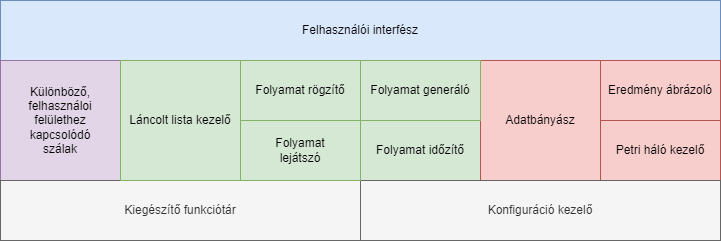
\includegraphics[width=\textwidth,keepaspectratio=true]{images/img_plan_1}
\label{fig:plan}
\end{center}
\end{figure}

\begin{itemize}
	\item \textbf{Felhasználói interfész}: A kezelőfelület, amivel a felhasználó eléri és kezelni tudja az egyes szoftverfunkciókat.
	\item \textbf{Felhasználói felülethez kapcsolódó szálak}:  Fontos - a felhasználó számára nem látható - szálak, amelyek feldata bizonyos billentyűkombinációk figyelése anélkül, hogy a program reszponzivitását kártékonyan befolyásolnák.
	\item \textbf{Láncolt lista kezelő}: Az egyes folyamatok láncolt listaként vannak kezelve a szoftverbe, ez az alrendszer felel a megfelelő értelmezésükért. 
	\item \textbf{Folyamat rögzítő}: Figyeli és rögzíti a perifériák általi beviteli értékeket.
	\item \textbf{Folymat generáló}: Előre meghatározott forgatóvkönyvek alapján úgy generál folyamatokat mintha azt egy felhasználó végezte volna el.
	\item \textbf{Folyamat lejátszó}: A folyamatokat játsza vissza, egy felhasználót szimulál.
	\item \textbf{Folyamat időzítő}: A Windowsba integrált rendszert felhasználva ütemez / időzít folyamatokat.
	\item \textbf{Adatbányász}: Az Alpha-algoritmust implementálva folyamatelemzést hajt végre több folyamaton.
	\item \textbf{Eredmény ábrázoló}: Az Adatbányász által elvégzett folyamatelemzés eredmé\hyp{}nyeit jeleníti meg.
	\item \textbf{Petri háló kezelő}: A petri-hálót mint struktúra, valamint a hozzátartozó függvé\hyp{}nyeket a szoftver számára értelmezhető módon implementálja.
	\item \textbf{Kiegészítő funkciótár}: Számos hasznos funkció gyűjteménye, melyet a többi alrendsze használ.
	\item \textbf{Konfiguráció kezelő}:  Futásidők között felhasználói preferenciák és beállítások tárolásáért és betöltéséért felel.
\end{itemize}

\Section{Az Alpha-algoritmus}

Az Alpha-algoritmust mint folyamatelemzési módszert hasznosan lehet alkalmazni a dolgozati témában. Az algoritmus, jelentőségét tekintve elengedhetetlen részét képezi a dolgozatnak. Jelen esetben a folyamatokat azok jellegétől és céljától függetlenül lehet elemezni, akár cél nélküli beviteli sorozatra is alkalmazható az Alpha-algoritmus.

\newpage
\subsection{Alkalmazása}

Ebben az alfejezetben bemutatásra kerül, hogy hogyan is kapcsolódik pontosan az Alpha-algoritmus a dolgozat témájához.
\newline

Az alább található példában három előre létrehozott folyamaton kerül alkalmazásra az Alpha-algoritmus. A folyamatok egyszerűek, hogy szemléletes legyen a példa, viszont ugyanezzel a módszerrel több száz vagy akár több ezer hosszú folyamaton is alkalmazha\hyp{}tó az algoritmus.
\newline

Maguk a folyamatok szolgálnak bemenetként, részeredményekként eseménynapló és lenyomati mátrix jön létre, kimentként pedig egy olyan petri háló kerül generálásra mely leírja a folyamat modelljét.

\begin{figure}[h]
\begin{center}
\caption{Beviteli folyamatok}
\begin{tabular}{|| c | c | c | c | c | c ||}
	\hline\hline
	\textbf{Folyamat} & \textbf{ID} & \textbf{Típus} & \textbf{Érték} & \textbf{Érték típusa} &  \textbf{Eltelt idő} \\ [0.5ex]
	\hline\hline
	1 & 1 & Key&  Left Alt & WM\_SYSKEYDOWN & 0 \\
	\hline
	1 & 2 & Key&  F4 & WM\_SYSKEYDOWN & 100 \\
	\hline
	1 & 3 & Key&  F4 & WM\_SYSKEYUP & 150 \\
	\hline
	1 & 4 & Key&  Left Alt & WM\_KEYUP & 612 \\
	\hline\hline
	2 & 1 & Key & Left Alt & WM\_SYSKEYDOWN & 0 \\
	\hline
	2 & 2 & Key & F4 & WM\_SYSKEYUP & 80 \\
	\hline
	2 & 3 & Key & F4 & WM\_SYSKEYDOWN & 51 \\
	\hline
	2 & 4 & Key & Left Alt & WM\_KEYUP & 152 \\
	\hline\hline
	3 & 1 & Key & Left Alt & WM\_SYSKEYDOWN & 0 \\
	\hline
	3 & 2 & Key & F12 & WM\_SYSKEYDOWN & 151 \\
	\hline
	3 & 3 & Key & Left Alt & WM\_KEYUP & 188 \\
	\hline\hline
\end{tabular}
\label{fig:planexample}
\end{center}
\end{figure}	

Az Alpha-algoritmus alkalmazásában, mint bármely folyamatbányászati algorit\hyp{}musnál, első lépésként ezekből az eseményekből fel kell építeni az eseménynaplót amiből később dolgozik az algoritmus. Ez a lépés konkrétan arról szól, hogy a már meglévő folyamatok az Alpha-algoritmusnak szükséges formátumra kerülnek átalakításra.

Ez jelen esetben az alábbi három szabály alapján történik:
\begin{enumerate}
	\item A "\textbf{Folyamat}" elnevezésű oszlop alapján triviális módon meghatározásra kerül az esethez tartozó egyedi azonosító,
	\item A "\textbf{Típus}", "\textbf{Érték}" és "\textbf{Érték típusa}" oszlophármas értékeiből létrejön a tevékenység megnevezése,  ami a továbbiakban \textit{,,Activity\_{x}"}-ként lesz feltüntetve,
	\item Az "\textbf{Eltelt idő}" oszlop alapján (az előző esemény óta eltelt időt mutatja) pedig létrejön egy relatív-időbélyeg az "\textbf{ID}" oszlop segítségével, hiszen az utóbbi alap\hyp{}ján határozható meg az események szekvenciája.
\end{enumerate}

\newpage

Ezeknek megfelelően az alábbi eseménynaplót kapjuk:

\begin{figure}[h]
\begin{center}
\caption{Eeseménynapló}
\begin{tabular}{|| c | c | c | c | c |  ||}
	\hline
	Azonosító & Tevékenység & Relatív időbélyeg \\ [0.5ex]
	\hline\hline
	1 & Activity\_0 & 0 \\
	\hline
	1 & Activity\_1 & 100 \\
	\hline
	1 & Activity\_2 & 250 \\
	\hline
	1 & Activity\_3 & 762 \\
	\hline
	2 & Activity\_0 & 0 \\
	\hline
	2 & Activity\_2 & 80 \\
	\hline
	2 & Activity\_1 & 131 \\
	\hline
	2 & Activity\_3 & 283 \\
	\hline
	3 & Activity\_0 & 0 \\
	\hline
	3 & Activity\_4 & 151 \\
	\hline
	3 & Activity\_3 & 339 \\
	\hline
\end{tabular}
\label{fig:planexample}
\end{center}
\end{figure}	

Miután megvan az eseménynapló, az Alpha-algoritmus elkezdei a munkát, azaz az eseménynaplót közvetlen-sorrend, okozat, párhuzam és választás relációkra alakítja, ezzel létrehozva az alábbi lenyomati mátrixot:

\begin{figure}[h]
\begin{center}
\caption{Lenyomati mátrix}
\begin{tabular}{|c | c | c | c | c | c|}
	\hline
	\hspace{0.1cm} & A\_0 & A\_1 & A\_2 & A\_3 & A\_4 \\
	\hline
	A\_0 & \# & $\rightarrow$ & $\rightarrow$ & \# & $\rightarrow$ \\
	\hline
	A\_1 & $\leftarrow$ & \# & $\parallel$ & $\rightarrow$ & \# \\
	\hline
	A\_2 & $\leftarrow$ & $\parallel$ & \# & $\rightarrow$ & \# \\
	\hline
	A\_3  & \# & $\leftarrow$ & $\leftarrow$ & \# & $\leftarrow$ \\
	\hline
	A\_4 & $\leftarrow$ & \# & \# & $\rightarrow$ & \# \\
	\hline
\end{tabular}
\label{fig:planexample}
\end{center}
\end{figure}

%	https://courses.edsa-project.eu/pluginfile.php/280/mod_resource/content/0/16%20Alpha%20Algorithm%20-%20A%20Process%20Discovery%20Algorithm.pdf



























